% ============================================================
%  雅思写作范文集 | IELTS Writing Notebook
%  编译器：XeLaTeX / Tectonic（见 ielts-writing/render.sh）
%  正文（Task 1 / Task 2 各主题）由 scripts/writing_db.py 自动生成，
%  请勿手动编辑两个 sentinel 注释之间的内容；preamble 可手改。
% ============================================================

\documentclass[12pt, a4paper]{article}

\usepackage{fontspec}
\usepackage{xeCJK}
\usepackage[top=2.5cm, bottom=2.5cm, left=2.8cm, right=2.8cm]{geometry}
\usepackage{xcolor}
\usepackage{mdframed}
\usepackage{titlesec}
\usepackage{fancyhdr}
\usepackage{enumitem}
\usepackage{graphicx}
\usepackage{soul}
\usepackage[hidelinks]{hyperref}

\setlength{\headheight}{15pt}

% ---------- 字体 ----------
\setmainfont{Times New Roman}
% 显式指定中文粗体字族（本地 XeLaTeX/Tectonic 不会自动配对 FandolSong 的两个 .otf）
\setCJKmainfont{FandolSong}[BoldFont={FandolSong Bold}]

% ---------- 颜色 ----------
\definecolor{headerblue}{RGB}{31, 73, 125}
\definecolor{promptbg}{RGB}{255, 247, 230}
\definecolor{promptborder}{RGB}{217, 152, 38}
\definecolor{samplebg}{RGB}{242, 242, 242}
\definecolor{sampleborder}{RGB}{150, 150, 150}
\definecolor{analysisbg}{RGB}{235, 247, 238}
\definecolor{analysisborder}{RGB}{60, 150, 90}
\definecolor{metacolor}{RGB}{120, 120, 120}
\definecolor{sourcecolor}{RGB}{102, 102, 153}
% 行文内「好表达」的高亮：浅黄底 + 加粗，醒目且不打断换行
\definecolor{hlbg}{RGB}{255, 241, 148}
\sethlcolor{hlbg}
% \hi{...} 标记范文/生成文中值得学习的表达
\newcommand{\hi}[1]{\texorpdfstring{\hl{\textbf{#1}}}{#1}}

% ---------- 页眉页脚 ----------
\pagestyle{fancy}
\fancyhf{}
\fancyhead[L]{\small\textcolor{headerblue}{\textbf{雅思写作范文集}}}
\fancyhead[R]{\small\textcolor{headerblue}{\nouppercase{\leftmark}}}
\fancyfoot[C]{\thepage}
\renewcommand{\headrulewidth}{0.4pt}

% ---------- 标题样式 ----------
\titleformat{\section}{\Large\bfseries\color{headerblue}}{}{0em}{}[\titlerule]
\titleformat{\subsection}{\large\bfseries\color{sourcecolor}}{}{0em}{}

% ---------- 框样式 ----------
\mdfdefinestyle{promptstyle}{
  backgroundcolor=promptbg, linecolor=promptborder, linewidth=1.2pt,
  topline=false, rightline=false, bottomline=false,
  innerleftmargin=10pt, innerrightmargin=10pt,
  innertopmargin=6pt, innerbottommargin=6pt, skipabove=8pt, skipbelow=6pt,
}
\mdfdefinestyle{samplestyle}{
  backgroundcolor=samplebg, linecolor=sampleborder, linewidth=1pt,
  topline=false, rightline=false, bottomline=false,
  innerleftmargin=10pt, innerrightmargin=10pt,
  innertopmargin=6pt, innerbottommargin=6pt, skipabove=6pt, skipbelow=6pt,
}
\mdfdefinestyle{analysisstyle}{
  backgroundcolor=analysisbg, linecolor=analysisborder, linewidth=1pt,
  topline=false, rightline=false, bottomline=false,
  innerleftmargin=10pt, innerrightmargin=10pt,
  innertopmargin=6pt, innerbottommargin=6pt, skipabove=6pt, skipbelow=6pt,
}

% ---------- 命令 / 环境定义 ----------

% \writingprompt{任务}{题型}{主题}{题目文字}
\newcommand{\writingprompt}[4]{%
  \begin{mdframed}[style=promptstyle]%
    \noindent{\small\bfseries\textcolor{promptborder}{#1}}%
    \enspace{\small\itshape\textcolor{metacolor}{#2}}%
    \enspace{\small\textcolor{metacolor}{[#3]}}%
    \par\vspace{3pt}%
    \noindent #4%
  \end{mdframed}%
}

% 参考范文框 / 亮点分析框
\newmdenv[style=samplestyle]{samplebox}
\newmdenv[style=analysisstyle]{analysisbox}

% \essaymeta{目标分数}{词数}
\newcommand{\essaymeta}[2]{%
  \par\vspace{4pt}%
  \noindent{\small\bfseries\textcolor{headerblue}{生成范文}}%
  \enspace{\small\textcolor{metacolor}{(目标 Band #1 · #2 words)}}%
  \par\vspace{3pt}%
}

% ============================================================
\begin{document}

% ===== 封面 =====
\begin{titlepage}
  \centering\vspace*{4cm}
  {\Huge\bfseries\color{headerblue} 雅思写作范文集}\\[0.5cm]
  {\Large IELTS Writing Notebook}\\[2cm]
  {\large Task 1 图表作文 \quad / \quad Task 2 议论文}\\[0.4cm]
  {\large 按任务类型与主题分类整理 · 目标 Band 8.5+}\\[2cm]
  {\large\textcolor{gray}{by zqy}}\\[0.5cm]
  {\large\textcolor{gray}{mason.zqy@gmail.com}}\\[3cm]
  \vfill
  {\large 开始日期：2026 年 6 月}
\end{titlepage}

\tableofcontents
\newpage

% >>> GENERATED BODY START — do not edit between the sentinels (writing_db.py rewrites this)

\section{Task 1：图表作文 (Academic Writing Task 1)}
\markboth{Task 1 图表作文}{}

\subsection{其他 (Other)}

\writingprompt{Task 1}{line}{其他 Other}{The graph below shows the consumption of three spreads (margarine, butter, and low fat and reduced spreads) from 1981 to 2007. Summarise the information by selecting and reporting the main features, and make comparisons where relevant.}

\begin{center}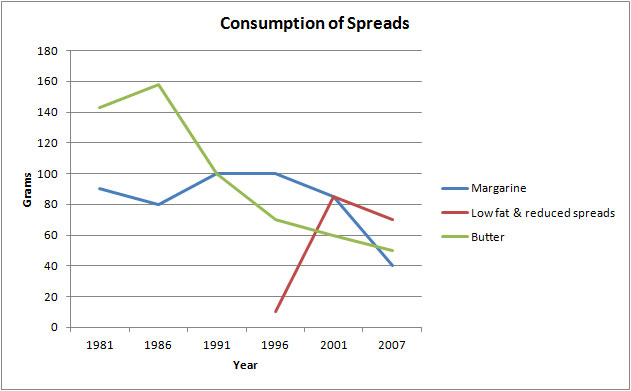
\includegraphics[width=0.9\linewidth,keepaspectratio]{images/task1-spreads-line-graph.jpg}\end{center}

\noindent\textbf{图表数据：}Butter: \textasciitilde{}140g (1981) → peak 160g (1986) → \textasciitilde{}50g (2007). Margarine: \textasciitilde{}90g (1981), fluctuating → \textasciitilde{}40g (2007). Low-fat \& reduced: begins 1996 at \textasciitilde{}10g → peak >80g (\textasciitilde{}2001) → \textasciitilde{}70g (2007). Units: grams.\par\vspace{4pt}

\begin{samplebox}
\textbf{参考范文} \textcolor{gray}{\small (来源：\href{https://ieltsliz.com/ielts-writing-task-1-line-graph-model-score-9/}{IELTS Liz — Line graph (spreads), Band 9})}\par\vspace{3pt}
The line graph illustrates the amount of three kinds of spreads (margarine, butter, and low fat and reduced spreads) which were consumed from 1981 to 2007. Units are measured in grams.

\par

Overall, \hi{the consumption of margarine and butter decreased over the period} given, while for low fat and reduced spreads, it rose. At the start of the period, butter was \hi{the most popular spread}. Margarine was the most widely consumed in the middle of the period but, by the end, low fat and reduced spreads was most popular.

\par

With regards to the amount of butter used, it began at around 140 grams and then \hi{peaked at} 160 grams in 1986 before \hi{falling dramatically} to about 50 grams in the last year. Likewise, approximately 90 grams of margarine was eaten in the first year, after which the figure \hi{fluctuated slightly} and dropped to a low of 40 grams in 2007.

\par

On the other hand, the consumption of low fats and reduced spreads only started in 1996 at about 10 grams. This figure, which \hi{reached a high of} just over 80 grams five years later, fell slightly in the final years to approximately 70 grams in 2007.
\end{samplebox}

\begin{analysisbox}
\textbf{亮点分析}\par\vspace{2pt}
This Band 9 report nails the two things examiners reward most in Task 1. First, it opens with a clear paraphrase of the rubric and then devotes a dedicated \hi{overview} paragraph to the big-picture trends without quoting specific numbers — the single most important move for Coherence and Task Achievement.

\par

Second, its Lexical Resource is built on a rich set of trend verbs and data phrases ("peaked at", "falling dramatically", "fluctuated slightly", "reached a high of") used accurately, so figures are reported with precision rather than a flat "went up / went down".
\vspace{3pt}\textbf{高分表达}\par
\begin{itemize}\setlength\itemsep{1pt}
\item \hi{peaked at} （达到峰值（为……）） \textcolor{gray}{——替代 reached the highest point}
\item \hi{fall dramatically} （急剧下降） \textcolor{gray}{——升级 decrease a lot}
\item \hi{fluctuate slightly} （小幅波动） \textcolor{gray}{——描述上下起伏}
\item \hi{reach a high of} （达到……的高点） \textcolor{gray}{——对应 drop to a low of}
\item \hi{over the period given} （在所给时间段内） \textcolor{gray}{——Task 1 概述常用时间状语}
\item \hi{plummet to} （骤降至） \textcolor{gray}{——比 fall 更强烈}
\item \hi{level/tail off} （趋平/逐渐减少） \textcolor{gray}{——描述末段放缓}
\end{itemize}
\end{analysisbox}

\essaymeta{8.5+}{169}

The line graph compares how much of three spreads — margarine, butter, and low-fat and reduced spreads — was consumed, in grams, between 1981 and 2007.

\par

Overall, \hi{the consumption of both butter and margarine declined markedly} over the period, whereas low-fat and reduced spreads, despite a later start, \hi{saw a steady rise}. Butter was initially the most popular, but by 2007 it had been overtaken by the low-fat alternative.

\par

In 1981, butter stood at roughly 140 grams and \hi{climbed to a peak of} 160 grams in 1986, before \hi{plummeting to} around 50 grams by the end of the period. Margarine followed a broadly similar downward trajectory, beginning near 90 grams, \hi{fluctuating slightly}, and \hi{bottoming out at} about 40 grams in 2007.

\par

By contrast, low-fat and reduced spreads were not introduced until 1996, when consumption stood at a mere 10 grams. The figure then \hi{surged to a high of} just over 80 grams within five years, before \hi{tailing off to} approximately 70 grams in the final year — making it the only spread whose consumption was higher at the end of the period than when it first appeared.

\vspace{10pt}\hrule height 0.2pt\vspace{10pt}


\section{Task 2：议论文 (Writing Task 2)}
\markboth{Task 2 议论文}{}

\subsection{科技 (Technology)}

\writingprompt{Task 2}{opinion}{科技 Technology}{Some people believe that technology has made man more social. To what extent do you agree or disagree with this opinion?}

\begin{samplebox}
\textbf{参考范文} \textcolor{gray}{\small (来源：\href{https://www.ieltspodcast.com/writing-task-2/band-9-sample-essays/technology-social/}{查看原文})}\par\vspace{3pt}
Experts throughout both the developing and developed world have debated whether \hi{the advent of sophisticated modern technology} such as mobile phones, laptops and iPads have helped to enhance and improve people's social lives or whether the opposite has become the case.

\par

Personally, I strongly advocate the former view. This essay will discuss both sides using examples from the UK government and Oxford University to demonstrate points and prove arguments.

\par

On the one hand there is ample, powerful, almost daily evidence that such technology can be detrimental especially to the younger generation who are more easily affected by its addictive nature and which can result in people feeling more isolated from society. The central reason behind this is twofold. Firstly, the invention of online social media sites and apps, such as Twitter and Facebook, have \hi{reduced crucial face-to-face interactions dramatically}. Through use of these appealing mediums, people feel in touch and connected yet lack key social skills and the ability to communicate. Secondly, dependence on such devices is built up frighteningly easily, which may have a damaging effect on mental health and \hi{encourage a sedentary lifestyle}.

\par

On the other hand, although there are significant downsides to technological developments, its multifold advantages cannot be denied. This is largely because the popularity of technology such as cellphones allows people to connect freely and easily \hi{with no geographical barriers}. People are able to share any type of news, information, photos and opinions with their loved ones whenever and wherever they want, therefore \hi{keeping a feeling of proximity and closeness}.

\par

From the arguments and examples given I firmly believe that overall communication and man's sociability has been advanced enormously due to the huge technological progress of the past twenty years and, despite some potentially serious health implications which governments should not fail to address, it is predicted that its popularity will continue to flourish in the future.
\end{samplebox}

\begin{analysisbox}
\textbf{亮点分析}\par\vspace{2pt}
This model answer scores well on Task Response and Coherence: it states a clear position early ("I strongly advocate the former view"), then devotes one body paragraph to each side with the discourse markers "On the one hand / On the other hand", and uses concrete (if invented) studies as support — a useful technique for adding specificity under exam conditions.

\par

Its real strength is Lexical Resource: precise, less-common collocations ("the advent of sophisticated modern technology", "detrimental to the younger generation", "encourage a sedentary lifestyle", "no geographical barriers") rather than generic vocabulary. Note, however, that the original contains several slips ("it's" for "its", "huge the huge") — at a genuine Band 8.5+ these would be ironed out, which is what my own version aims to do while reusing the strongest phrasing.
\vspace{3pt}\textbf{高分表达}\par
\begin{itemize}\setlength\itemsep{1pt}
\item \hi{the advent of sophisticated modern technology} （先进现代科技的出现/到来） \textcolor{gray}{——升级 the appearance of new technology}
\item \hi{be detrimental to} （对……有害） \textcolor{gray}{——替代 be bad for}
\item \hi{reduce crucial face-to-face interactions} （减少关键的面对面交流） \textcolor{gray}{——讨论社交/科技题常用}
\item \hi{encourage a sedentary lifestyle} （助长久坐不动的生活方式） \textcolor{gray}{——健康/科技题高分搭配}
\item \hi{with no geographical barriers} （没有地理障碍） \textcolor{gray}{——替代 from anywhere}
\item \hi{keep a feeling of proximity and closeness} （维持亲近感） \textcolor{gray}{——描写远程沟通维系关系}
\item \hi{hollow out the quality of those connections} （掏空/削弱这些联系的质量） \textcolor{gray}{——我的范文用法，强调深度受损}
\end{itemize}
\end{analysisbox}

\essaymeta{8.5+}{268}

It is frequently claimed that modern digital technology has rendered humanity more sociable than ever before. While I accept that such tools have undeniably widened our networks of contact, I would argue that they have simultaneously \hi{hollowed out the quality of those connections}, making the assertion only partially true.

\par

There is certainly compelling evidence that technology has expanded our social reach. Instant-messaging platforms and video-calling applications allow individuals to \hi{sustain relationships across vast geographical distances} that would once have severed them entirely. A student studying overseas, for instance, can now converse face to face with family members on a daily basis, thereby preserving a sense of closeness that previous generations could scarcely have imagined. In this respect, the sheer breadth of human contact has grown exponentially.

\par

Nevertheless, this proliferation of contact should not be mistaken for genuine sociability. For many people, the convenience of communicating through a screen has displaced the richer interactions that occur in person, fostering relationships that are \hi{wide but shallow}. Adolescents in particular may accumulate hundreds of online acquaintances while struggling to sustain a meaningful conversation in the physical world. Moreover, the addictive design of social media frequently encourages solitary, sedentary scrolling rather than collective activity, leaving users paradoxically more isolated despite being \hi{perpetually connected}.

\par

In conclusion, while I acknowledge that technology has multiplied the opportunities for people to stay in touch, I only partially agree that it has made us more social, since the depth and authenticity of our relationships have arguably been diluted in the process. The real challenge lies in harnessing these tools to \hi{complement, rather than replace, face-to-face human connection}.

\vspace{10pt}\hrule height 0.2pt\vspace{10pt}

% <<< GENERATED BODY END

\end{document}
